\section{Resultados}
% Metodologia de testes, testes efectuados (make some stuff up, para não ser só um teste? aquilo é perfeitamente linear por isso é fácil) e resultados
\paragraph{}
Com a introdução de N processadores, teoricamente, espera-se obter um \textit{speedup} de N em relação à implementação com apenas 1 processador. Esta expectativa assume que a introdução de mais processadores resulta numa execução completamente em paralelo, que não existem \textit{overheads} de paralelização e que não existem limitações no acesso a recursos partilhados pelos processadores.

No desenvolvimento desta aplicação tentou-se a utilização de 2, 4, 8 e 12 processadores. Os resultados obtidos encontram-se nas tabelas abaixo.

\begin{table}[H]
\centering
\begin{tabular}{c|ccc|cc}

\# Processadores            & 448 bytes & 52741 bytes & 1235204 bytes & Speed Up & Eficiência \\
\hline
1 & 15 & 1765 & 41357 & 1 & 1  \\
2 & 8 & 891 & 20703 & 1.95 & 0.98  \\
4 & 4 & 448 & 10361 & 3.89 & 0.97  \\
8 & 3 & 253 & 5896 & 6.33 & 0.79  \\
12 &  & Não testado & & &  \\
\end{tabular}
\caption{Resultados}
\end{table}

\begin{figure}[H]
\centering
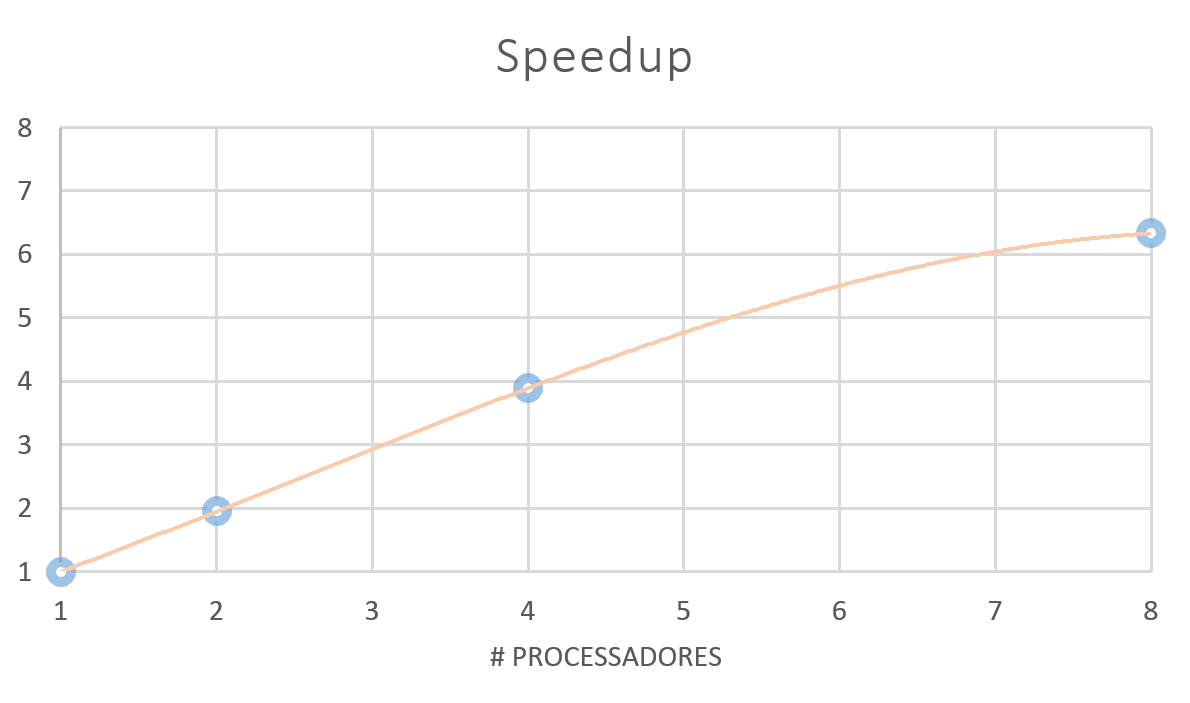
\includegraphics[width=140mm]{SpeedUp.PNG}
\caption{Speed Up \label{Speed Up}}
\end{figure}

\begin{figure}[H]
\centering
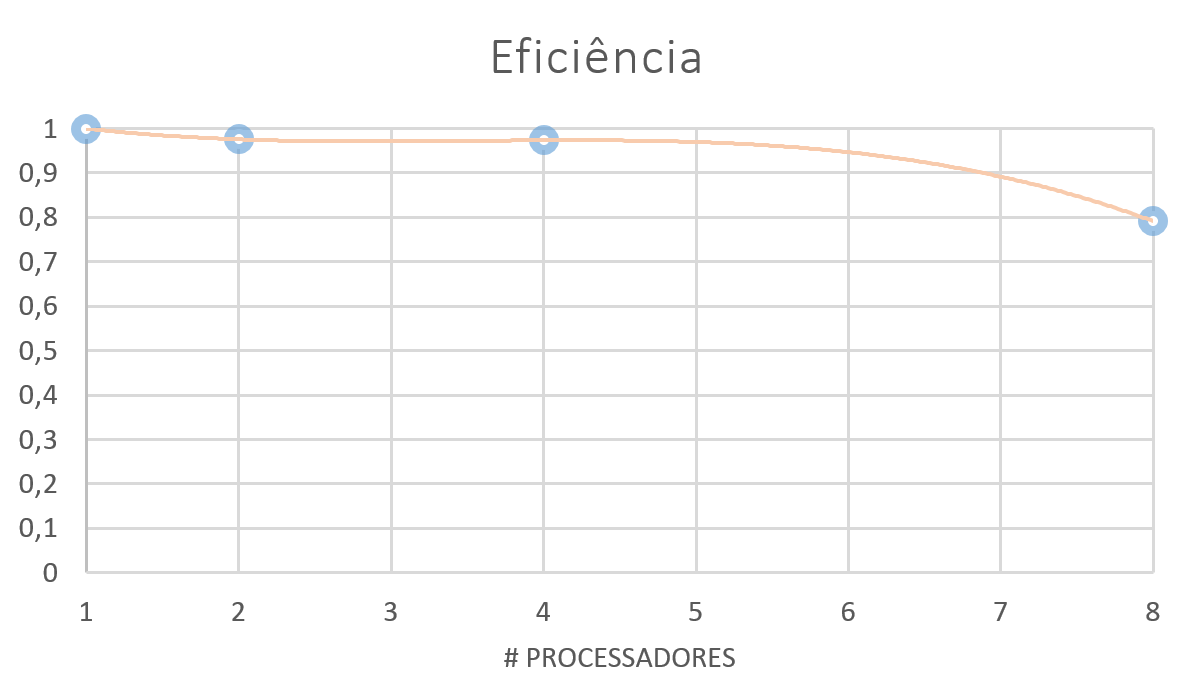
\includegraphics[width=140mm]{Eficiencia.PNG}
\caption{Eficiência \label{Eficiencia}}
\end{figure}

Numa fase inicial optou-se por fazer uma implementação apenas com 2 processadores para garantir que as técnicas utilizadas para implementar a distribuição de dados e a sincronização entre processadores funcionavam correctamente. Tal como se esperava, obteve-se um \textit{speedup} de 2 em relação à implementação só com um processador, para ambos os testes com o ficheiro pequeno e com o ficheiro grande.

De seguida experimentou-se utilizar 4 processadores e os resultados obtidos continuaram de acordo com o esperado uma vez que o \textit{speedup} obtido para ambos os testes foi aproximadamente 4.

Com a introdução de 8 processadores os resultados obtidos já não foram de acordo com o esperado, pois os \textit{speedups} obtidos são consideravelmente mais reduzidos do que o esperado.

Antes de se tentar gerar o \textit{bitstream} do hardware com 12 processadores foram feitas algumas contas para garantir que o número de BRAMs disponíveis era suficiente para as necessidades de memória da aplicação e chegou-se à conclusão que estas eram garantidas. Quando se tentou gerar o \textit{bitstream} do hardware verificou-se então que o número de LUTs da FPGA era demasiado reduzido para gerar o \textit{hardware} e por isso não foi possível testar o funcionamento com 12 processadores.

Com a posterior análise do relatório de síntese da implementação com 8 processadores concluiu-se que esta ocupava 99\% do número de \textit{slices} da FPGA, desta forma concluiu-se que este seria o limite máximo de processadores que poderiam ser utilizados na FPGA utilizada no laboratório.

A partir dos resultados obtidos concluiu-se que a teoria definida inicialmente não é verificada na prática para qualquer número de processadores. Até 4 processadores os resultados obtidos foram muito próximos do esperado, mas para quantidades superiores os resultados começam a afastar-se do ideal. Isto deve-se aos \textit{overheads} de paralelização, que incluem principalmente o sincronismo e as limitações no acesso a recursos partilhados, nomeadamente a memória externa que é acedida constantemente por todos os processadores.

No caso da aplicação implementada os \textit{overheads} de paralelização são muito reduzidos e por isso a maior limitação de escalabilidade encontra-se na arbitragem do acesso à memória de dados. Estes resultados estão de acordo com as limitações referidas na secção de Limitações do Hardware.

